\chapter[Simulação e desenho experimental]{Simulação física, estatísticas quadráticas e desenho experimental}
\label{chap:simulacao}

Este capítulo define o experimento gerador e verifica os momentos dos
seus dados sintéticos. A resposta tensorial validada anteriormente é
combinada com espectros de sinal e ruído para gerar coeficientes complexos
de resíduos. As estatísticas antes e depois da compressão são obtidas das
mesmas realizações. O resultado é uma implementação verificável
desse experimento; ainda não são calculados posteriors, cobertura ou
limites de massa.

\section{Experimento periódico e normalização dos dados}

Considera-se uma duração \(T\), com frequências positivas
\(f_n=n/T\), \(n=1,\ldots,K\). O experimento é definido diretamente
por blocos de Fourier independentes, sem ajuste do modelo de temporização
ou janela que misture canais. Para cada frequência,
\begin{equation}
 q_n\sim\mathcal{CN}(0,C_n),\qquad
 \langle q_nq_m^\dagger\rangle=\delta_{nm}C_n,\qquad
 \langle q_nq_m^T\rangle=0.
 \label{eq:sim-cn}
\end{equation}
A última igualdade define a propriedade da distribuição complexa. A
matriz \(C_n\) tem unidades de espectro unilateral de resíduos,
\(\mathrm{s}^3\). Com coeficientes de série
\(a_n=q_n/\sqrt{2T}\), a reconstrução real é
\begin{equation}
 r_a(t)=\sqrt{\frac2T}\,\operatorname{Re}
       \sum_{n=1}^{K}q_{na}e^{i2\pi f_nt}.
 \label{eq:sim-serie}
\end{equation}
Logo, \([q]=\mathrm{s}^{3/2}\) e \([r]=\mathrm{s}\).
A convenção conserva a parte imaginária da correlação cruzada definida
no capítulo anterior. O sinal global comum da resposta de redshift se
cancela na geração por covariância; a conjugação de apenas um dos fatores
não seria permitida.

A covariância é construída como
\begin{equation}
 C_{n,ab}=P_{\rm gw}(f_n)\Gamma_{ab}(f_n)
 +\delta_{ab}\left[
       \rho_a^2P_{\rm red}(f_n)
       +2(E\sigma_a)^2\Delta t\right].
 \label{eq:sim-covariancia}
\end{equation}
Aqui \(\sigma_a\) é a incerteza nominal dos tempos de chegada,
\(E\) é um fator comum de ruído branco e \(\rho_a\) é um padrão
relativo de amplitudes de ruído vermelho, fixado no desenho. O fator
\(2\sigma^2\Delta t\) é o espectro unilateral do ruído branco de uma
grade regular. Quando apenas três canais são retidos, a série
\eqref{eq:sim-serie} contém somente essa banda: não representa um ruído
branco independente em todos os instantes da grade.

Para sinal e ruído vermelho, utiliza-se
\begin{equation}
 P(f;A,\gamma)=\frac{A^2}{12\pi^2f_{\rm piv}^3}
                  \left(\frac{f}{f_{\rm piv}}\right)^{-\gamma},
 \qquad f_{\rm piv}=\frac1{\text{ano juliano}}.
 \label{eq:sim-espectro}
\end{equation}
Essa convenção é consistente com o espectro de resíduos do capítulo
anterior. O pivô que define a amplitude não é a frequência
\(f_{\rm ref}=1/T\) utilizada na aproximação da resposta. Sinal,
amplitude vermelha, inclinação do sinal e fator de ruído branco são
parâmetros variáveis do modelo, e não uma única amplitude ajustada a uma
curva média.

A geração usa \(C_n=L_nL_n^\dagger\) e
\(q_n=L_n(x_n+iy_n)/\sqrt2\), com componentes normais padrão
independentes. Matrizes inválidas são rejeitadas; não se recortam
autovalores. Para estabilizar unidades, divide-se \(C_n\) por uma
escala positiva \(s_n\), definida por parâmetros fiduciais fixados antes
da injeção. O coeficiente armazenado é
\(\bar q_n=q_n/\sqrt{s_n}\). Os valores de \(s_n\) integram o
arquivo de resultados e permanecem constantes ao avaliar parâmetros.
As fórmulas seguintes utilizam as covariâncias e coeficientes
normalizados, de modo que as estatísticas são adimensionais.

\section{Estimadores angulares e propagação exata dos momentos}

Os pares são orientados por \(a<b\). Sua separação define quatro
grupos com números de pares tão iguais quanto possível, e cada grupo
recebe pesos uniformes. São conservadas as partes real e imaginária dos
produtos cruzados, produzindo oito estimadores. Dois grupos de autos,
definidos pela ordenação das incertezas nominais \(\sigma_a\), completam
um vetor real de dimensão dez. Não se adiciona uma auto imaginária,
identicamente nula. Geometria, binagem e pesos são fixados antes dos
sorteios, sem utilizar potências observadas ou a verdade injetada.

Cada estimador tem a forma
\begin{equation}
 y_{ni}=\bar q_n^\dagger H_i\bar q_n,\qquad H_i=H_i^\dagger.
 \label{eq:sim-quadratica}
\end{equation}
Para a parte real de um par, os elementos fora da diagonal são
\(H_{ab}=H_{ba}=1/2\). Para
\(\operatorname{Im}(\bar q_a\bar q_b^*)\), são
\(H_{ab}=i/2\) e \(H_{ba}=-i/2\). Os pesos do grupo multiplicam
esses elementos. A aplicação da identidade de Isserlis para uma
normal complexa própria fornece
\begin{equation}
 \mu_{ni}=\operatorname{tr}(H_i\bar C_n),\qquad
 \Sigma_{n,ij}=\operatorname{tr}
                   (H_i\bar C_nH_j\bar C_n).
 \label{eq:sim-momentos}
\end{equation}
Não há o fator dois da expressão análoga para formas quadráticas de
vetores reais. Os testes confrontam essa expressão com uma construção
independente das covariâncias complexas dos pares, preservando inclusive
as covariâncias entre partes reais e imaginárias.

Na compressão de frequência são utilizados pesos fixos \(w_n\):
\begin{equation}
 y_{B,i}=\sum_nw_ny_{ni},\qquad
 \mu_{B,i}=\sum_nw_n\mu_{ni},\qquad
 \Sigma_{B,ij}=\sum_nw_n^2\Sigma_{n,ij}.
 \label{eq:sim-compressao}
\end{equation}
A última igualdade depende da independência dos canais do experimento
atual. A operação geral, implementada separadamente, é
\(\mu_B=W\mu_A\), \(\Sigma_B=W\Sigma_AW^T\), conservando
blocos entre frequências quando presentes. A mesma operação atua nos
dados, na média e na covariância previstas.

\section{Distribuição das estatísticas e controle pareado}

Um campo gaussiano não torna gaussianas suas estatísticas quadráticas.
Para uma projeção escalar com matriz \(H\), a cumulante de ordem
\(r\) é
\begin{equation}
 \kappa_r=(r-1)!\operatorname{tr}[(H\bar C)^r].
 \label{eq:sim-cumulantes}
\end{equation}
Se \(\lambda_j\) são os autovalores de
\(L^\dagger HL\), a curtose excessiva é
\begin{equation}
 \gamma_2=6\frac{\sum_j\lambda_j^4}
                    {(\sum_j\lambda_j^2)^2}>0
 \label{eq:sim-curtose}
\end{equation}
para toda projeção não degenerada. Em um canal, ela é ao menos
\(6/N_p\). A compressão de canais independentes soma as cumulantes
com pesos \(w_n^r\), podendo reduzir, mas não anulando necessariamente,
a assimetria ou a curtose.

Além das estatísticas físicas, gera-se um controle
\begin{equation}
 y_n^{G}\sim\mathcal N(\mu_n,\Sigma_n).
 \label{eq:sim-controle}
\end{equation}
O controle utiliza coordenadas normais dos mesmos sorteios latentes do
gerador complexo, preservando as duas distribuições marginais. Essa
associação permite identificar as realizações correspondentes, mas não
implica igualdade dos experimentos ou garantia de redução de variância.
A compressão do controle usa o mesmo \(W\). No controle G, a família
normal de A/B é exata; nos dados físicos, continua sendo uma aproximação
que exigirá calibração própria.

A análise A0 futura utilizará diretamente os coeficientes complexos, com
\begin{equation}
 \log p(q\mid\theta)=
 -\sum_n\left[q_n^\dagger C_n^{-1}q_n+
             \log\det C_n+N_p\log\pi\right].
 \label{eq:sim-a0}
\end{equation}
A utilizará os vetores quadráticos por frequência e uma normal com
momentos \eqref{eq:sim-momentos}; B utilizará sua compressão fixa.
Comparar A e B nos dados físicos exige separar a alteração da
compressão de uma eventual falha da aproximação normal. O controle G
foi criado precisamente para distinguir essas questões.

\subsection{Duas definições da aproximação em frequência}

Definem-se separadamente os modelos
\begin{align}
 \Gamma^{C_{\rm full}}_n
 &=\Gamma\bigl(\beta(f_{\rm ref}),2\pi f_{\rm ref}L/c\bigr),
 \label{eq:sim-cfull}\\
 \Gamma^{C_\beta}_n
 &=\Gamma\bigl(\beta(f_{\rm ref}),2\pi f_nL/c\bigr).
 \label{eq:sim-cbeta}
\end{align}
A notação representa todas as distâncias da matriz. O primeiro congela a
velocidade e as fases dos pulsares; o segundo conserva as fases de cada
canal. Ambos recebem exatamente os dados comprimidos de B, com média e
covariância recalculadas. Espectro, ruídos e escalas de normalização não
são congelados pela aproximação da resposta.

Em massa nula, \(C_\beta\) coincide com B, enquanto
\(C_{\rm full}\) pode diferir por conservar fases da frequência de
referência. Portanto, uma diferença entre B e \(C_{\rm full}\) não
pode ser atribuída exclusivamente à aproximação da dispersão. No
recorte inicial, \(u=f_gT\in[0,1]\), todos os canais permanecem
viajantes. Nenhuma observação é removida ao variar u; um componente
evanescente exigiria outra definição do modelo.

\section{Configurações executadas e verificação de momentos}

A referência auditada utiliza dez direções sintéticas em uma esfera de
Fibonacci, duração de 15 anos, três canais positivos e uma grade ideal
de 392 instantes, com cadência aproximada de 13,9764 dias. As distâncias
são fixadas entre 100 e 300 anos-luz, e as incertezas nominais entre 100
e 500 nanossegundos. Trata-se de uma geometria reduzida para validar
momentos, sem pretensão de reproduzir uma PTA observada ou
representativa. O maior \(fL/c\) é 60, dentro do domínio validado da resposta.

O caso massivo usa \(u=0{,}6\),
\(\log_{10}A_{\rm gw}=-14{,}9\), \(\gamma_{\rm gw}=4{,}1\),
\(\log_{10}A_{\rm red}=-15{,}3\), \(\gamma_{\rm red}=4\)
e \(E=1{,}1\). Há também um controle com \(u=0\) e esses mesmos
espectros, e um controle de ruído branco sem sinal gravitacional ou
ruído vermelho. O arquivo JSON representa amplitudes exatamente nulas
por \texttt{null}, traduzido internamente como
\(\log_{10}A=-\infty\). Os pesos de frequência são \(1/3\), e a
normalização fiducial utiliza \(\log_{10}A=-14{,}7\),
\(\gamma=13/3\) e a mediana das incertezas nominais.

Cada configuração contém 128 blocos independentes de 1024 realizações,
totalizando 131072 sorteios físicos e seus controles. As sementes são
691206, 691207 e 691208 para massivo, GR e apenas ruído,
respectivamente. Os erros-padrão Monte Carlo são estimados entre os
blocos. Verificam-se a média de Fourier, a covariância completa inclusive
entre canais, a pseudocovariância, as médias e covariâncias de A/B físicas
e normais, e cumulantes selecionadas. O limiar empírico pré-fixado é de
seis erros-padrão; não constitui um teorema de cobertura simultânea.

\begin{center}
\begingroup\small\singlespacing
\begin{tabular}{@{}lrrr@{}}
\toprule
Configuração & Pares verificados & Maior discrepância MC & Tempo total (s)\\
\midrule
Massiva & 275 & \(3{,}502\) & \(21{,}76\)\\
GR & 165 & \(3{,}936\) & \(15{,}93\)\\
Apenas ruído & 165 & \(3{,}187\) & \(15{,}96\)\\
\bottomrule
\end{tabular}
\endgroup
\end{center}
Os números de pares contam as entradas superiores, incluindo autos,
das matrizes distintas necessárias a B, \(C_{\rm full}\) e
\(C_\beta\). Entradas exatamente idênticas são reutilizadas. A maior
diferença entre os controles numéricos de ORF foi
\(3{,}12\times10^{-13}\). O custo inclui construir as respostas e
verificar momentos, antes da serialização, nesta máquina. Os três casos
foram executados simultaneamente, com outras tarefas concorrentes; os
tempos refletem essa carga e não estimam uma campanha de inferência.

As matrizes de ORF massivas apresentaram menor autovalor de
aproximadamente \(0{,}2951\), e a maior parte imaginária absoluta foi
\(0{,}00430\). A maior condição espectral das covariâncias massivas
foi aproximadamente 4,33. Os testes unitários adicionais verificaram
unidades e reconstrução por Fourier, as identidades de Isserlis, o
operador de compressão, o tratamento da pseudocovariância, os argumentos
de \(C_{\rm full}\)/\(C_\beta\) e a recusa de entradas ou
resoluções inválidas. Onze testes passaram.

A validação não sustenta normalidade das estatísticas físicas. Por
exemplo, no primeiro bin de autos do caso massivo, a teoria fornece
assimetria \(1{,}0227\) e curtose excessiva \(1{,}6831\) no primeiro
canal. Após a compressão, os valores são \(0{,}6324\) e
\(0{,}6641\). O acordo das estimativas com esses valores confirma a
persistência de cumulantes não gaussianas. No controle G, as mesmas
medidas são compatíveis com zero dentro da incerteza Monte Carlo.

A Figura~\ref{fig:simulacao-nao-normalidade} ilustra essa distinção com
sorteios adicionais, separados das campanhas da tabela.
\begin{figure}[htbp]
 \centering
 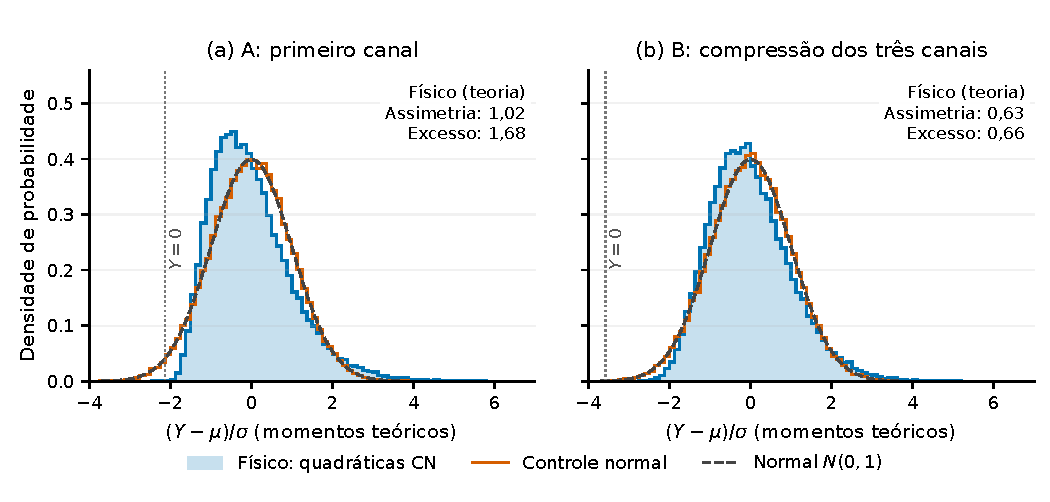
\includegraphics[width=\textwidth]{../figures/C06/nao_normalidade.pdf}
 \caption{Não normalidade do primeiro grupo de autos na configuração
 massiva: primeiro canal de A e compressão B dos três canais com pesos
 iguais. Os histogramas usam 65\,536 realizações novas por experimento,
 semente 2026091066, e padronização pela média e variância teóricas.
 A curva tracejada é a normal padrão; a linha vertical indica o auto
 físico nulo. As anotações mostram assimetria e excesso de curtose
 teóricos. Os autos negativos do controle normal foram mantidos.
 As densidades usam o número total de sorteios, incluindo os pontos
 fora da janela.}
 \label{fig:simulacao-nao-normalidade}
\end{figure}

No caso massivo, substituir B por \(C_{\rm full}\) altera a média
comprimida em até \(0{,}605\) desvio-padrão marginal e sua covariância
em aproximadamente 24\% na norma de Frobenius relativa. Esses são
deslocamentos condicionais de momentos em uma injeção; não são viés de
posterior, perda de informação ou falha de cobertura. No controle GR,
\(C_\beta\) coincide com B, e o pequeno deslocamento de
\(C_{\rm full}\) confirma que congelar fases é uma aproximação
adicional.

\section{Precisão numérica e alcance do modelo}

O adaptador de referência utiliza a validação da resposta tensorial para
todos os pares. As resoluções comuns são
\((\ell_{\max},N_\mu^{h},N_\mu^{d},N_\varphi^{d})=
(460,900,500,1000)\) e \((520,1000,600,1200)\). São preservados os
relatórios de refinamento, erro por par e soma conservadora dos
erros da matriz. Produtos escalares de direções já verificadas
como unitárias são saturados em \([-1,1]\) somente para remover
arredondamento. Não há recorte de autovalores ou interpolação em massa.

Essa implementação auditada é apropriada para pequenas referências,
mas não deve recalcular a integral angular para cada avaliação de uma
likelihood. O cálculo das campanhas de inferência reutiliza
coeficientes harmônicos de cada pulsar entre todos os pares, construir
matrizes em nós explícitos de massa e controlar separadamente a
quadratura de parâmetros e da ORF. Uma rede ideal com 12 pulsares,
quatro canais, \(T=4{,}5\) ou 15 anos e distâncias entre 300 e 1000
anos-luz conserva \(fL/c\leq888{,}89\). Esses limites têm significado
físico declarado e mantêm o custo dentro do envelope já auditado;
valores típicos maiores exigem ampliar a validação ou definir médias
em distância e frequência. Tal ampliação não foi executada neste
capítulo.

Os cinco parâmetros iniciais previstos para inferência são
\[
(u,\log_{10}A_{\rm gw},\gamma_{\rm gw},
\log_{10}A_{\rm red},\log_{10}E).
\]
Degenerações de massa, amplitude
e espectro, sensibilidade às prioris e dependência efetiva dos resultados
dos dados devem ser medidas. SBC requer injeções sorteadas da priori;
cobertura condicional requer injeções fixas e novos dados. A calibração mantém a distinção entre
validação por simulações da priori e diagnóstico dependente dos dados
\cite{talts2018,modrak2025}: postos marginais, isoladamente, podem deixar
passar um algoritmo que devolve a própria priori. O desenho prospectivo
e seus limites de parâmetros estão registrados em arquivo de configuração.
Os blocos de Monte Carlo empregados
para verificar momentos são novos experimentos sintéticos, e não
segmentos independentes artificialmente atribuídos a uma única PTA.

Uma janela irregular ou um ajuste de temporização pode acoplar modos e
produzir pseudocovariância \(P=\langle qq^T\rangle\ne0\). Nesse caso,
\begin{equation}
 \operatorname{Cov}\begin{pmatrix}\operatorname{Re}q\\
                                  \operatorname{Im}q\end{pmatrix}
 =\frac12\begin{pmatrix}
  \operatorname{Re}(C+P)&\operatorname{Im}(P-C)\\
  \operatorname{Im}(P+C)&\operatorname{Re}(C-P)
 \end{pmatrix}.
 \label{eq:sim-cov-real}
\end{equation}
A conversão é disponibilizada, mas não há implementação de janela ou
ajuste neste experimento. A likelihood CN própria e os momentos
\eqref{eq:sim-momentos} não podem ser transferidos sem correção para
esse domínio. As configurações e os procedimentos de reprodução são disponibilizados no material suplementar.
